\section{FPGAs}
\begin{figure}
\centering
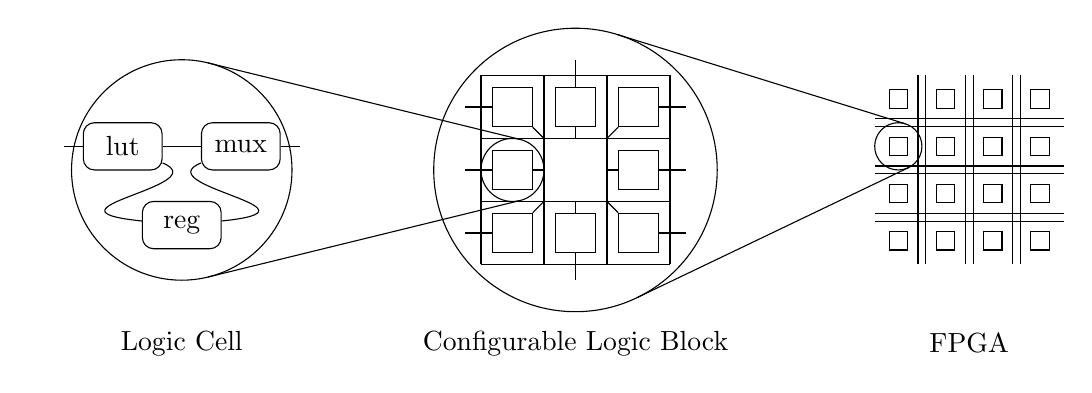
\begin{tikzpicture}
	\pgfmathsetmacro{\xone}{0}
	\pgfmathsetmacro{\xtwo}{5}
    \pgfmathsetmacro{\xthree}{10}
    
    \node [circle, draw] (cone) at (\xone,1.7) [minimum size=2.8cm] {};
    \node [circle, draw] (ctwo) at (\xtwo-0.8, 1.7) [minimum size=0.8cm] {};
\draw (0.33333333333333326, 3.0597385369580756)--(4.295238095238095, 2.0884967248451645);
\draw (0.33333333333333326, 0.34026146304192406)--(4.295238095238095, 1.3115032751548354);

    
    \draw (\xtwo, 1.7) circle (1.8cm);
    \draw (\xthree-0.9, 1.7+0.3) circle (0.3cm);
    \draw (5.532729751800444, 3.4193600587272686)--(9.18878829196674, 2.286560009787878);
\draw (5.777329419797189, 0.07649792943841183)--(9.229554903299531, 1.7294163215730687);
    
    \draw (\xone, -0.5) node {Logic Cell};
    \draw (\xtwo, -0.5) node {Configurable Logic Block};
    \draw (\xthree, -0.5) node {FPGA};


	\draw (\xone-0.75,2) node[rectangle, rounded corners, draw=black,minimum height=0.6cm, minimum width=1cm] (lut) {lut};
	\draw (\xone,1) node[rectangle, rounded corners, draw=black,minimum height=0.6cm, minimum width=1cm] (reg) {reg};
	\draw (\xone+0.75,2) node[rectangle, rounded corners, draw=black,minimum height=0.6cm, minimum width=1cm] (mux) {mux};
	
	\draw (lut)..controls (\xone+0.45,1.5) and (\xone-1.95, 1.2)..(reg);
	\draw (mux)..controls (\xone-0.45,1.5) and (\xone+1.95, 1.2)..(reg);
	\draw (lut)--(mux);
	\draw (lut)--(\xone-1.5,2);
	\draw (mux)--(\xone+1.5,2);
	
	

	
	
	\draw (\xtwo-0.8, 2.5) node[rectangle, draw=black, minimum height = 0.5cm, minimum width=0.5cm] (n1) {};
	
	\draw (\xtwo, 2.5) node[rectangle, draw=black, minimum height = 0.5cm, minimum width=0.5cm] (n2) {};
	
	\draw (\xtwo+0.8, 2.5) node[rectangle, draw=black, minimum height = 0.5cm, minimum width=0.5cm] (n3) {};
	
	\draw (\xtwo-0.8, 1.7) node[rectangle, draw=black, minimum height = 0.5cm, minimum width=0.5cm] (n4) {};
	
	\draw (\xtwo+0.8, 1.7) node[rectangle, draw=black, minimum height = 0.5cm, minimum width=0.5cm] (n5) {};
	
	\draw (\xtwo-0.8, 0.9) node[rectangle, draw=black, minimum height = 0.5cm, minimum width=0.5cm] (n6) {};
	
	
	\draw (\xtwo, 0.9) node[rectangle, draw=black, minimum height = 0.5cm, minimum width=0.5cm] (n7) {};
	
	
	\draw (\xtwo+0.8, 0.9) node[rectangle, draw=black, minimum height = 0.5cm, minimum width=0.5cm] (n8) {};
	
	\draw(\xtwo-1.2,2.9)--(\xtwo-1.2,0.5);
	\draw(\xtwo-0.4,2.9)--(\xtwo-0.4,0.5);
	\draw(\xtwo+0.4,2.9)--(\xtwo+0.4,0.5);
	\draw(\xtwo+1.2,2.9)--(\xtwo+1.2,0.5);
	
	\draw(\xtwo-1.2,2.9)--(\xtwo+1.2,2.9);
    \draw(\xtwo-1.2,2.1)--(\xtwo+1.2,2.1);
    \draw(\xtwo-1.2,1.3)--(\xtwo+1.2,1.3);
    \draw(\xtwo-1.2,0.5)--(\xtwo+1.2,0.5);
    
    %Lines from logic cells to the inside
    \draw(n1)--(\xtwo-0.4,2.1);
    \draw(n2)--(\xtwo,2.1);
    \draw(n3)--(\xtwo+0.4,2.1);
    \draw(n4)--(\xtwo-0.4,1.7);
    \draw(n5)--(\xtwo+0.4,1.7);
    \draw(n6)--(\xtwo-0.4,1.3);
    \draw(n7)--(\xtwo,1.3);
	\draw(n8)--(\xtwo+0.4,1.3);
	
   %Lines from logic cells to the outside;
   \draw(n1)--(\xtwo-1.4, 2.5);
   \draw(n2)--(\xtwo, 3.1);
   \draw(n3)--(\xtwo+1.4, 2.5);
   \draw(n4)--(\xtwo-1.4, 1.7);
   \draw(n5)--(\xtwo+1.4, 1.7);
   \draw(n6)--(\xtwo-1.4, 0.9);
   \draw(n7)--(\xtwo, 0.3);
   \draw(n8)--(\xtwo+1.4, 0.9);
   
   
   \draw (\xthree-0.9, 1.7+0.9) node[rectangle, draw=black] (sn1) {};
   \draw (\xthree-0.3, 1.7+0.9) node[rectangle, draw=black] (sn2) {};
   \draw (\xthree+0.3, 1.7+0.9) node[rectangle, draw=black] (sn3) {};
   \draw (\xthree+0.9, 1.7+0.9) node[rectangle, draw=black] (sn4) {};   
   
   \draw (\xthree-0.9, 1.7+0.3) node[rectangle, draw=black] (sn5) {};
   \draw (\xthree-0.3, 1.7+0.3) node[rectangle, draw=black] (sn6) {};
   \draw (\xthree+0.3, 1.7+0.3) node[rectangle, draw=black] (sn7) {};
   \draw (\xthree+0.9, 1.7+0.3) node[rectangle, draw=black] (sn8) {};
   
   \draw (\xthree-0.9, 1.7-0.3) node[rectangle, draw=black] (sn9) {};
   \draw (\xthree-0.3, 1.7-0.3) node[rectangle, draw=black] (sn10) {};
   \draw (\xthree+0.3, 1.7-0.3) node[rectangle, draw=black] (sn11) {};
   \draw (\xthree+0.9, 1.7-0.3) node[rectangle, draw=black] (sn12) {};
   
   \draw (\xthree-0.9, 1.7-0.9) node[rectangle, draw=black] (sn13) {};
   \draw (\xthree-0.3, 1.7-0.9) node[rectangle, draw=black] (sn14) {};
   \draw (\xthree+0.3, 1.7-0.9) node[rectangle, draw=black] (sn15) {};
   \draw (\xthree+0.9, 1.7-0.9) node[rectangle, draw=black] (sn16) {};
   
   \draw (\xthree-0.05, 1.7+1.2)--(\xthree-0.05, 1.7-1.2);
   \draw (\xthree+0.05, 1.7+1.2)--(\xthree+0.05, 1.7-1.2);
   \draw (\xthree+0.6-0.05, 1.7+1.2)--(\xthree+0.6-0.05, 1.7-1.2);
   \draw (\xthree+0.6+0.05, 1.7+1.2)--(\xthree+0.6+0.05, 1.7-1.2);
   \draw (\xthree-0.6-0.05, 1.7+1.2)--(\xthree-0.6-0.05, 1.7-1.2);
   \draw (\xthree-0.6+0.05, 1.7+1.2)--(\xthree-0.6+0.05, 1.7-1.2);
   
   \draw (\xthree+1.2, 1.7+0.05)--(\xthree-1.2, 1.7+0.05);
   \draw (\xthree+1.2, 1.7-0.05)--(\xthree-1.2, 1.7-0.05);
   \draw (\xthree+1.2, 1.7+0.6+0.05)--(\xthree-1.2, 1.7+0.6+0.05);
   \draw (\xthree+1.2, 1.7+0.6-0.05)--(\xthree-1.2, 1.7+0.6-0.05);
   \draw (\xthree+1.2, 1.7-0.6+0.05)--(\xthree-1.2, 1.7-0.6+0.05);
   \draw (\xthree+1.2, 1.7-0.6-0.05)--(\xthree-1.2, 1.7-0.6-0.05);

	
\end{tikzpicture}
\caption{The hierarchy of a typical FPGA. A typical FPGA mostly consists of Configurable Logic Blocks (CLBs), and a CLB mostly consists of logic cells. The way logic cells and CLBs are connected may be different for each FPGA architecture.}
\end{figure}


The computing hardware most people are familiar with is CPUs. Manufacturers incorporate them in every desktop pc, laptop, and most mobile devices. CPUs are very flexible and efficient- which is why they are the de facto standard for any computation task. In CPU computation, an integrated circuit (a processor) iteratively reads an instruction from a RAM module (in the form of encoded bits), performs the instruction, and then continues to read the next instruction. The instructions are not embedded in the circuit of the CPU itself.

FPGAs are different from CPUs, as they do not store the programs they execute in RAM- they instead configure them in the (highly parallel) logic of the circuit itself. Configuring an FPGA to execute a specific program entails loading a configuration file onto the hardware and restarting the FPGA such that it reconfigures its logic. The hardware will then perform the configured logic on the input it receives via IO pins. 

Because each logic cell performs logic independently, FPGAs can perform computations highly parallel and without delays from sequentially loading instructions. This computation process implies that FPGAs are very efficient at executing concurrent programs. Reconfiguring an FPGA is, however, a relatively expensive operation. Therefore, FPGAs are unsuitable for changing from program to program, as a CPU does when running an operating system. Moreover, FPGAs can be slower than CPUs for nonparallel applications since its longer critical path length (i.e. distance an electric current has to travel each clock cycle) results in a lower clock speed. Lastly, the different structure of an FPGA requires programs for them to be developed in specialised HDL languages instead of CPU-based programming languages. However, efforts are being made to bring these domains closer together.

FPGAs perform execution using components such as lookup tables, registers, and special-purpose modules\footnote{These modules are used for efficient storage or calculation of specific functions. We will disregard them in this research.}. These components are physical structures on the circuit. In the next sections, we will discuss these modules.
\subsection{Lookup tables}


\begin{figure}
\centering
\begin{tabular}{|c|c|c|}
\hline
$p$ & $q$ & $p$ XOR $q$ \\ \hline
$F$ & $F$ & $F$       \\ \hline
$F$ & $T$ & $T$       \\ \hline
$T$ & $F$ & $T$       \\ \hline
$T$ & $T$ & $F$       \\ \hline
\end{tabular}
\caption{A truth table that shows the result of an XOR operation}
\label{fig:truth_table}
\end{figure}

\begin{figure}
\centering
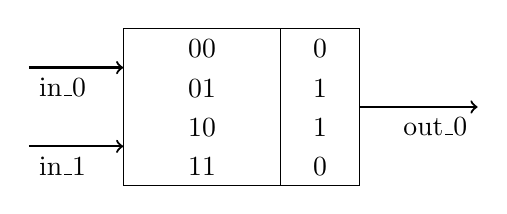
\begin{tikzpicture}
    \draw (0,0) rectangle (3,2);
    \draw (2, 0) -- (2, 2);
    \draw[thick,->] (-1.2,0.5) node[anchor=north west] {in\_1} -- (0,0.5);
    \draw[thick,->] (-1.2,1.5) node[anchor=north west] {in\_0} -- (0,1.5);
    
    \draw[thick,->] (3,1)  -- (4.5,1) node[anchor=north east] {out\_0};
    
    \draw[draw=white] (1,1.5)    node[anchor=south] {00};
    \draw[draw=white] (1,1)      node[anchor=south] {01};
    \draw[draw=white] (1,0.5)    node[anchor=south] {10};
    \draw[draw=white] (1,0)      node[anchor=south] {11};
    
    
    \draw[draw=white] (2.5,1.5)   node[anchor=south] {$0$};
    \draw[draw=white] (2.5,1)     node[anchor=south] {$1$};
    \draw[draw=white] (2.5,0.5)   node[anchor=south] {$1$};
    \draw[draw=white] (2.5,0)     node[anchor=south] {$0$};
\end{tikzpicture}
\caption{A Lookup Table (LUT) in which an XOR-operation is configured}
\label{fig:lookuptable}
\end{figure}

Any boolean logic formula can be expressed in the form of a truth table, such as in Figure \ref{fig:truth_table}. The leftmost column of a truth table specifies all possible combinations of $T$ and $F$ for all inputs; the rightmost column then specifies what output that specific logic function would give. Each distinct combination of $T$ and $F$ in the rightmost column corresponds to a different boolean formula. FPGAs execute logic in the form of Lookup Tables (LUTs), which model the evaluation of a truth table, but with ones and zeroes instead of $T$ and $F$: for every combination of ones and zeroes in the input, the LUT stores what output it should give. The compilation software provided by the FPGA vendor can reconfigure these outputs. This way, any boolean formula with the appropriate number of variables can be implemented with a lookup table. Figure \ref{fig:lookuptable} shows a lookup table that has two input bits and one output bit. This lookup table is configured to perform an XOR-operation. Lookup tables can have input and output consisting of any number of bits, depending on the FPGA design.

\subsection{Registers}
\begin{figure}
\centering
\begin{tikzpicture}
    \draw (0,0) rectangle (1.5,2);
    \draw[-{Latex[length=5mm, open]}] (-1.2,0.5) node [anchor=north west] {$clock$} -- (0.5,0.5);
    \draw[-{Latex[length=3mm]}] (-1.2,1.5) node[anchor=east] {$D$} -- (0,1.5);
    
    \draw (-1.2,1.6) -- (-0.8,1.6) -- (-0.5,1.5);
    \draw (-1.2,1.7) -- (-0.8,1.7) -- (-0.5,1.5);

    \draw (1.5, 1.1)--(1.9,1.1)--(2.2,1);
    \draw (1.5, 1.2)--(1.9,1.2)--(2.2,1);
    \draw[-{Latex[length=3mm]}] (1.5,1) -- (2.7,1) node[anchor=west] {$Q$};
\end{tikzpicture}
\caption{Traditional representation of a register. Note that input \textit{D} and output \textit{Q} may consist of multiple wires.}
\label{fig:register}
\end{figure}

Programs require intermediate data storage to perform any computation that is more complex than combinational logic. FPGAs use registers for this purpose (see Figure \ref{fig:register}). Registers can store a small collection of bits, depending on the FPGA design. When a register's input $clock$ changes from 0 to 1, the contents of the register are replaced by the value of the input $D$, and the output $Q$ takes the value of the previous content. The output stays constant until the clock changes from 0 to 1 again when D has a different value.

FPGAs usually have clocks- wires whose signal constantly changes between 0 and 1 that is connected to registers in the hardware. These clocks can be a single global clock connected to each register or a network of clocks each responsible for different parts of the FPGA. The frequency of this clock is chosen such that all signals are guaranteed to be stable when the clock becomes 1. This stability is very convenient for programmers, who do not have to calculate the time it takes for a signal to propagate through a wire. The implication is that each circuit combining only lookup tables that end in the D-input of a register takes the same amount of time.

If the FPGA program has longer chains of lookup tables, then it takes longer for the output signal to stabilise. The vendor software accommodates for this by setting the global clock at a lower frequency. Since programs on FPGAs are highly parallel, there are likely some parts of the calculation that do not require a lower clock speed and can cause slowdown because of this. In these scenarios, adding registers to some parts of an FPGA program can improve performance if it allows the global clock speed to be higher.


\subsection{Logic cells}

\begin{figure}
\centering
\begin{tikzpicture}
	%Register
    \draw (0,0) rectangle (1.5,2);
    \draw[-{Latex[length=5mm, open]}] (-1.2,-1) node [anchor=south east] {$clock$} -- (-1.2,0.5) -- (0.5,0.5);
    
    %Line from Register to MUX
    \draw[-{Latex[length=3mm]}] (1.5,1) -- (2.7,1) -- (2.7, 2.333) -- (3.7, 2.333);
    \draw (1.5, 1.1) -- (1.9, 1.1) -- (2.1, 1);
    \draw (1.5, 1.2) -- (1.9, 1.2) -- (2.1, 1);
    \draw (2.56,1) -- (2.7, 1.14);
    \draw (2.42,1) -- (2.7, 1.28);
    \draw (2.7, 2.1933) -- (2.84, 2.333);
    \draw (2.7, 2.0533) -- (2.98, 2.333);
    
    %LUT
    \draw (-5,2) rectangle (-2,4);
    \draw (-3, 2) -- (-3, 4);

    \draw[-{Latex[length=3mm]}] (-6.5,3) node[anchor=north west] {in} -- (-5,3);
	\draw (-6.5, 3.1) -- (-6.1, 3.1);
	\draw (-6.5, 3.2) -- (-6.1, 3.2);
	\draw (-6.1, 3.1) -- (-5.9, 3);
	\draw (-6.1, 3.2) -- (-5.9, 3);
    
    
    
    %Line from LUT to Register
    \draw[-{Latex[length=3mm]}] (-2,3)  -- (-1.1,3) -- (-1.1, 1.5) -- (0,1.5);
	
	\draw (-2,3.1) -- (-1.6,3.1) -- (-1.4, 3);    
	\draw (-2,3.2) -- (-1.6,3.2) -- (-1.4, 3);

    \draw (-1.24, 3) -- (-1.1, 2.86);
    \draw (-1.38, 3) -- (-1.1, 2.72);
    \draw (-1.1, 1.64) -- (-0.96, 1.5);
    \draw (-1.1, 1.78) -- (-0.82, 1.5);
    
    
    %LUT keys
    \draw[draw=white] (-4,3.25) node[anchor=south] {$0000$};
    \draw[draw=white] (-4,2.75) node[anchor=south] {$\cdots$};
    \draw[draw=white] (-4,2.25) node[anchor=south] {$1111$};
    
    %LUT values
    \draw[draw=white] (-2.5,3.25) node[anchor=south] {$x_0$};
    \draw[draw=white] (-2.5,2.75) node[anchor=south] {$\cdots$};
    \draw[draw=white] (-2.5,2.25) node[anchor=south] {$x_n$};
    
    %Line from LUT to MUX
    \draw[-{Latex[length=3mm]}] (-2,3)  -- (3.7,3);
    
    %MUX
    \draw (3.7, 3.6667) -- (3.7, 1.6667) -- (4.7, 2.111) -- (4.7, 3.111) -- cycle;
    
    %M
    \draw[-{Latex[length=3mm]}] (2.2, 0.5) node[anchor=north west] {$m$} --(4.2, 0.5) -- (4.2, 1.8667);
    
    
    \draw[-{Latex[length=3mm]}] (4.7, 2.5) -- (6.2, 2.5) node[anchor = north east] {out};
    \draw (4.7, 2.6) -- (5.1, 2.6);
    \draw (4.7, 2.7) -- (5.1, 2.7);
    \draw (5.1, 2.6) -- (5.3, 2.5);
    \draw (5.1, 2.7) -- (5.3, 2.5);      

    
\end{tikzpicture}
\caption{An $n$-input logic cell. $x_k$ and $m$ must be configured for any $0 \leq k \leq n$}
\label{fig:logiccell}
\end{figure}

A typical logic cell is a combination of one or more lookup tables, a register, and a MUX (a 3-input gate that outputs a copy of the first or second input, depending on the value of the third input).  The contents of the lookup tables can be configured to perform any logic operation, and the value of the third MUX-input can be configured to specify whether the computation is clocked/synchronous or combinatorial/asynchronous. A logic cell is shown in Figure \ref{fig:logiccell}. Unfortunately for us, vendors have different logic cell designs, meaning we cannot generalise this example.

FPGA manufacturers often group Logic cells in Configurable Logic Blocks (CLB) that make hardware production, placement, and routing (Section \ref{sec:compilation}) easier.
 
The main building blocks of FPGAs are CLBs that are connected via routing fabric. These are responsible for most of the computation of FPGA programs. FPGAs can have additional modules such as RAM and Digital Signal Processors that optimise storage and specialised arithmetic, respectively. Each of these modules' functionality could also be performed by a collection of logic cells at the cost of performance. In this research, we will only consider CLBs.

\subsection{Routing}
A single logic cell can only perform simple programs such as logic gates. The FPGA needs to connect different logic cells to perform any kind of logic operation, dependent on what program it needs to execute. The way logic cells and other modules are connected on a physical FPGA in a specific configuration is called the \textbf{routing} of an FPGA. On the most basic level, FPGAs perform routing with configurable transistors. These are tiny modules on an FPGA board that are connected with an input wire and an output wire. They can be configured to allow electric current flowing from its input to its output or to block any incoming electric current.

\subsection{Pins}
To supply the FPGA with input and to allow it to provide output, an FPGA is equipped with a set of metal pins. Each of those pins is connected with a wire on the FPGA board. Each pin can be used for either input or output, depending on the configured program. For example, an FPGA used to control an electric stepper motor will receive input with the requested motor speed and direction and will output signals to specific circuits that need to be activated to obtain that speed and direction.




\section{FPGA compilation}
\label{sec:compilation}
To program an FPGA, an engineer has to specify a hardware design that describes the semantics of the program. They write these hardware designs in a Hardware Description Language (HDL). Commonly used languages for this purpose are VHDL and Verilog. They specify on an abstract level what functionality the program should have, preferably in a modular structure to improve maintainability.

The software then needs to translate this abstract description to a \textbf{netlist}: a description of logic, registers, specialised components, and how they are connected. Depending on the configuration of the compilation software, this netlist may undergo a sequence of optimisations and transformations between several levels of abstraction. This process is called \textbf{synthesis}; beware though that some sources call the entire FPGA compilation process synthesis.

The next step in the compilation process is \textbf{placement}. The software maps each LUT, register, and other components to a physical place on the FPGA. The software can place components closer together to optimise the speed or can place components further apart to increase the probability routes can be found. Finding the optimal placement for speed is a proven NP-hard problem.

The last step in the compilation process is \textbf{routing}. State-of-the-art FPGA compilation pipelines perform this step sequentially after placement\cite{alhyari2019}. With the components locked in place, the software attempts to find a configuration of routing switches such that each connection that the synthesis requires is made. Finding the optimal routes for speed is an NP-hard problem while finding any matching routing configuration is an NP problem. Both can be reduced to the problem of fixed-vertex subgraph homeomorphism of which the optimisation variant needs to explore the entire search tree, which \cite{ExactComplexity} showed can be computed in $O(2^{|T|-|S|}n^{O(1)})$ for the general case. However, routing algorithms are often made for specific FPGA architectures, allowing for better heuristics and thus performance.

\begin{minipage}{\textwidth}
\begin{important}
Note that place \& route of an FPGA \textit{program} as described here is a very similar problem to the emulation an unconfigured virtual FPGA to a concrete FPGA (this research). However, it is important to note that these are different problems: with place \& route, a mapping is obtained from a model of an \textit{FPGA program} to the concrete FPGA. In our research, we obtain a mapping from a model of a \textit{virtual FPGA} to the concrete FPGA. The two problems are on different levels of abstraction: an FPGA program does not have the concept of unconfigured components or transistors while a virtual FPGA does.

\vspace{.6cm}
Placement of FPGA programs using place \& route could theoretically also work on a higher abstraction level, i.e. including unconfigured components. The problem with this approach is that state-of-the art place \& route pipelines perform these algorithms sequentially: they perform placement based on speed- and routeability heuristics without a guarantee that the placement can indeed be routed \cite{alhyari2019}. With the placement of FPGA programs, this is not a problem. They are usually modular with components that have relatively few interconnecting wires. FPGAs, however, can consist of densely connected components that can severely impact routeability. We leave the analysis of place \& route algorithms for compatibility with FPGA-on-FPGA emulation for future research.
\end{important}
\end{minipage}


\begin{figure}
    \centering
\begin{tikzpicture}
    \draw (0,0) rectangle (3,2);
    \draw (2, 0) -- (2, 2);
    \draw[thick,->] (-1.2,0.5) node[anchor=north west] {in\_2} -- (0,0.5);
    \draw[thick,->] (-1.2,1.5) node[anchor=north west] {in\_1} -- (0,1.5);
    
    \draw[thick,->] (3,1)  -- (4,1) node[anchor=north] {out\_1};
    
    \draw[draw=white] (1,1.5)     node[anchor=south] {00};
    \draw[draw=white] (1,1)       node[anchor=south] {01};
    \draw[draw=white] (1,0.5)     node[anchor=south] {10};
    \draw[draw=white] (1,0)       node[anchor=south] {11};
    
    
    \draw[draw=white] (2.5,1.5)    node[anchor=south] {$x_0$};
    \draw[draw=white] (2.5,1)      node[anchor=south] {$x_1$};
    \draw[draw=white] (2.5,0.5)    node[anchor=south] {$x_2$};
    \draw[draw=white] (2.5,0)      node[anchor=south] {$x_3$};
    
    

     \draw (8,-1) rectangle (11,3);
    \draw (10, -1) -- (10, 3);
    \draw[thick,->] (6.8,0) node[anchor=north west] {in\_2} -- (8,0);
    \draw[thick,->] (6.8,1) node[anchor=north west] {N/A} -- (8,1);    
    \draw[thick,->] (6.8,2) node[anchor=north west] {in\_1} -- (8,2);
    
    \draw[thick,->] (11,1.5)  -- (12,1.5) node[anchor=north] {out\_1};
    \draw[thick,->] (11,0.5)  -- (12,0.5) node[anchor=north] {0};
    
	\draw[draw=white] (9,2.5)        node[anchor=south] {000};
    \draw[draw=white] (9,2)          node[anchor=south] {001};    
    \draw[draw=white] (9,1.5)        node[anchor=south] {010};
    \draw[draw=white] (9,1)          node[anchor=south] {011};
    \draw[draw=white] (9,0.5)        node[anchor=south] {100};
    \draw[draw=white] (9,0)          node[anchor=south] {101};
    \draw[draw=white] (9,-0.5)        node[anchor=south] {110};
    \draw[draw=white] (9,-1)          node[anchor=south] {111};
    
    
    \draw[draw=white] (10.5,2.5)         node[anchor=south] {$x_0 0$};
    \draw[draw=white] (10.5,2)           node[anchor=south] {$x_1 0$};    
    \draw[draw=white] (10.5,1.5)         node[anchor=south] {$x_0 0$};
    \draw[draw=white] (10.5,1)           node[anchor=south] {$x_1 0$};
    \draw[draw=white] (10.5,0.5)         node[anchor=south] {$x_2 0$};
    \draw[draw=white] (10.5,0)           node[anchor=south] {$x_3 0$};
    \draw[draw=white] (10.5,-0.5)         node[anchor=south] {$x_2 0$};
    \draw[draw=white] (10.5,-1)           node[anchor=south] {$x_3 0$};
    
    \draw[vecArrow] (5.5,1) -- (6.5,1);

\end{tikzpicture}
    \caption{Emulation of an FPGA: the configuration of the virtual FPGA is reflected in the configuration of the concrete FPGA. Any extra inputs and outputs are unused.}
    \label{fig:emulation}
    \vspace{1cm}
    \begin{tikzpicture}
    \draw (0,0) rectangle (3,2);
    \draw (2, 0) -- (2, 2);
    \draw[thick,->] (-1.2,0.5) node[anchor=north west] {in\_2} -- (0,0.5);
    \draw[thick,->] (-1.2,1.5) node[anchor=north west] {in\_1} -- (0,1.5);
    
    \draw[thick,->] (3,1)  -- (4,1) node[anchor=north west] {out\_1};
    
    \draw[draw=white] (1,1.5)    node[anchor=south] {00};
    \draw[draw=white] (1,1)      node[anchor=south] {01};
    \draw[draw=white] (1,0.5)    node[anchor=south] {10};
    \draw[draw=white] (1,0)      node[anchor=south] {11};
    
    
    \draw[draw=white] (2.5,1.5)     node[anchor=south] {$x_0$};
    \draw[draw=white] (2.5,1)       node[anchor=south] {$x_1$};
    \draw[draw=white] (2.5,0.5)     node[anchor=south] {$x_2$};
    \draw[draw=white] (2.5,0)       node[anchor=south] {$x_3$};
    
    

    \draw (8,-1.5) rectangle (11,2);
    \draw (10, -1.5) -- (10, 2);
	
	\draw[thick,->] (6.8,1.9) node[anchor=north west] 	{$x_0$} -- (8,1.9);
	\draw[thick,->] (6.8,1.3) node[anchor=north west] 	{$x_1$} -- (8,1.3);
	\draw[thick,->] (6.8,0.7) node[anchor=north west] 	{$x_2$} -- (8,0.7);
	\draw[thick,->] (6.8,0.1) node[anchor=north west] 	{$x_3$} -- (8,0.1);
	\draw[thick,->] (6.8,-0.5) node[anchor=north west] 	{in\_1} -- (8,-0.5);
    \draw[thick,->] (6.8,-1.1) node[anchor=north west] 	{in\_2} -- (8,-1.1);

    
    \draw[thick,->] (11,1)  -- (12,1) node[anchor=north west] {out\_1};
    
    \draw[draw=white] (9,1.5)       node[anchor=south] {000000};
    \draw[draw=white] (9,1)         node[anchor=south] {000001};
    \draw[draw=white] (9,0.5)       node[anchor=south] {000010};
	\draw[draw=white] (9,0)         node[anchor=south] {$\cdots$};
    \draw[draw=white] (9,-0.5)      node[anchor=south] {111101};
    \draw[draw=white] (9,-1) 	    node[anchor=south] {111110};
    \draw[draw=white] (9,-1.5)      node[anchor=south] {111111};
    
    
    
    \draw[draw=white] (10.5,1.5)         node[anchor=south] {$0$};
    \draw[draw=white] (10.5,1)           node[anchor=south] {$0$};
    \draw[draw=white] (10.5,0.5)         node[anchor=south] {$0$};
	\draw[draw=white] (10.5,0)           node[anchor=south] {$\cdots$};
	\draw[draw=white] (10.5,-0.5)        node[anchor=south] {$1$};
	\draw[draw=white] (10.5,-1)          node[anchor=south] {$1$};
	\draw[draw=white] (10.5,-1.5)        node[anchor=south] {$1$};
    
    
    \draw[vecArrow] (5.5,1) -- (6.5,1);

\end{tikzpicture}
    \caption{An FPGA virtual machine: the programming of the virtual FPGA is reflected in \textit{additional input} of the actual FPGA originating from some explicit configuration source, e.g. RAM or a storage device connected to the concrete FPGA's input pins. The configuration of the concrete FPGA does \textit{not} depend on the configuration of the virtual FPGA and additional logic- and storage resources are used.}
    \label{fig:simulation}
\end{figure}

\section{The FPGA virtual machine}
\label{sec:simulation}
In this research, we will not be implementing an FPGA virtual machine. However, for clarity, we will explain what we mean by it. Imagine a software engineer wants to execute a program $P$. Conventionally, they would program $P$ in an HDL, compile it to an FPGA configuration file and load it onto the hardware.

To instead simulate the synthesised program, the engineer can also program a generic FPGA environment in an HDL, compile it to an FPGA configuration file and load it onto the hardware. They can afterwards provide $P$ as \textit{input} to the program instead of using $P$ \textit{as} a program. This way, the virtual FPGA can run in a ``virtual machine" on the concrete FPGA. The \textit{static} configuration of the virtual FPGA uses the \textit{dynamic} resources (e.g. RAM and registers) of the concrete FPGA. A virtual machine of a single LUT is shown in Figure \ref{fig:simulation}.

Although engineers could use FPGA virtual machines to execute FPGA programs on FPGA hardware that the FPGA software was not compiled for, it introduces a considerable delay in execution. After all, many more dynamic components on the FPGA need to be used to store and execute the configuration of the same program.	



\section{FPGA emulation}
Instead, our research entails finding out how we can perform \textit{emulation}. With this, we mean the execution of a program on a different FPGA \textit{such that no extra input is required.} Instead, the emulator software inspects the program for the virtual FPGA and generates what program on the concrete FPGA would have the same semantics given the same inputs as the source FPGA. Figure \ref{fig:emulation} shows the emulation counterpart of Figure \ref{fig:simulation} with a smaller LUT. Since the target FPGA has one more input than the virtual FPGA, that input remains unused. Similarly, since it has one more output, that output remains unused (i.e. always outputs 0). The configuration of the LUT is such that it has the same semantics as the virtual LUT with these constraints in mind. We aim to find out how we can perform this kind of emulation with any program with any fixed source- and destination FPGA whenever such emulation is possible.
